\documentclass[xcolor={x11names,svgnames}]{beamer}

\usepackage[french]{babel}
\usepackage[T1]{fontenc}
\usepackage{cellspace}

\usepackage{amsmath}
\usepackage{amsfonts}
\usepackage{tikz}
\usepackage{xspace}
%\usepackage[absolute,overlay]{textpos}
\usepackage[normalem]{ulem}
\usepackage{minted}

%\usepackage{eurosym}
\usepackage{marvosym}
\usepackage{pifont}
\usepackage{xcolor}

\newcommand{\bigO}[1]{\ensuremath{\mathcal{O}\left( #1 \right)} }

\newcommand{\red}{\alert}
\newcommand{\green}{\color{LimeGreen}}
\newcommand{\blue}{\color{cyan}}

% FORTIN
\newcommand{\mynote}[1]{\note<1>[item]{#1}}
\newcommand{\euro}{\EUR\xspace}

\usetikzlibrary{patterns}
\usetikzlibrary{snakes}
 \usetikzlibrary{arrows}
\usetikzlibrary{backgrounds}
\usetikzlibrary{shapes}
\usetikzlibrary{shadows}
\usetikzlibrary{calc}
\usetikzlibrary{decorations}
\usetikzlibrary{decorations.pathmorphing}
\usetikzlibrary{decorations.shapes}
\usetikzlibrary{decorations.markings}
\usetikzlibrary{positioning}

\definecolor{amethyst}{rgb}{0.6, 0.4, 0.8}
\definecolor{cyan}{rgb}{0,0.6796875,1}

\usecolortheme{rose}
\setbeamertemplate{footline}{}
\setbeamertemplate{navigation symbols}{}

\usepackage{fontspec}

\setsansfont{PalatinoSansLTPro}[
   Path = /home/charles/charles_work/fonts/PalatinoSans/, 
   Extension      = .otf,
   UprightFont    = *-Regular,
   BoldFont= *-Bold ,
   ItalicFont = *-Italic,
   BoldItalicFont = *-BoldIta
]

\author[C.~Bouillaguet]{Charles Bouillaguet \newline
  {\small (\texttt{charles.bouillaguet@univ-lille.fr})}}

\title{Cours 2.5 : MPI suite}
\date{2021-02-12}

\begin{document}

\section{Introduction}

\begin{frame}[label=title]
  \titlepage
\end{frame}

%%%%%%%%%%%%%%%%%%%%%%%%%%%%%%%%%%%%%%%%%%%%%%%%%%%%%%%%%%%%%%%%

\begin{frame}
\frametitle{Durée des communications ?}

\begin{block}{Envoi d'un message du rang $i$ au rang $j$}
  \[
    T = \alpha + n \times \beta
  \]
  
  \begin{itemize}
  \item $n =$ taille des données (bit)
  \item $\alpha =$ \alert{latence} (s)
  \item $\beta \approx$ \alert{débit} (s / bit).
  \end{itemize}
\end{block}

\medskip

$1 / \beta$ : bit / s (\alert{bande passante}).

\medskip

\begin{alertblock}{Modèle \textbf{simplifié} et \textbf{optimiste} !}
\begin{itemize}
\item $T$ indépendant de $i$ et $j$ (topologie ?)
\item Indépendant des autres envois (congestion ?)
\end{itemize}
\end{alertblock}

\end{frame}

%%%%%%%%%%%%%%%%%%%%%%%%%%%%%%%%%%%%%%%%%%%%%%%%%%%%%%%%%%%%%%%

\begin{frame}[fragile]
\frametitle{MPI : simple et efficace}

\begin{minted}[fontsize=\small]{C}
int MPI_Send(const void* buf, int count, MPI_Datatype datatype,
             int dest, int tag, MPI_Comm comm);

int MPI_Recv(void* buf, int count, MPI_Datatype datatype,
             int source, int tag, MPI_Comm comm,
             MPI_Status *status);
\end{minted}

\bigskip

\footnotesize 
\begin{tabular}{|c|c|c|l|r|r|}
  \hline
  Cluster & Site & Année & Interface & Bandwith & Latency \\
  \hline
  \hline
  PPTI      & jussieu & 20?? & \phantom{00}1Gbit ethernet &   64Mo/s & 50.0$\mu$s \\
  sagitaire & lyon  & 2006 & \phantom{00}1Gbit ethernet   &   116Mo/s & 65.0$\mu$s \\
  \pause
  taurus    & lyon  & 2012 & \phantom{0}10Gbit ethernet   &  1156Mo/s & 25.9$\mu$s\\
  \pause
  gros      & nancy & 2019 & \phantom{0}25Gbit ethernet   &  2480Mo/s & 8.9$\mu$s\\
  \hline
  \pause
  grcinq    & nancy & 2013 & \phantom{0}56Gbit InfiniBand &  2488Mo/s & 1.2$\mu$s \\
  \pause
  grimoire  & nancy & 2016 & \phantom{0}56Gbit InfiniBand &  4248Mo/s & 1.1$\mu$s\\
  \pause
  drac      & grenoble & 2015 & 100Gbit InfiniBand  & 7760Mo/s & 1.7$\mu$s \\
  \hline
  \pause
  grvingt   & nancy & 2018 & 100Gbit OmniPath  & 12100Mo/s & 0.9$\mu$s \\
  \hline
\end{tabular}
(mesure : ping-pong entre deux noeuds)
\end{frame}

%%%%%%%%%%%%%%%%%%%%%%%%%%%%%%%%%%%%%%%%%%%%%%%%%%%%%%%%%%%%%%%%

\begin{frame}[fragile]
\frametitle{MPI : fonctions utiles}

\begin{minted}[fontsize=\small]{C}
double MPI_Wtime();
\end{minted}
               
\bigskip

Secondes écoulées depuis un point quelconque du passé, avec beaucoup
de chiffres significatifs (mesure précise).
\end{frame}


%%%%%%%%%%%%%%%%%%%%%%%%%%%%%%%%%%%%%%%%%%%%%%%%%%%%%%%%%%%%%%%%%

\begin{frame}[fragile]
\frametitle{MPI : échange de message}

Solution naïve (\mintinline{C}{MPI_Send} puis \mintinline{C}{MPI_Send}) $\leadsto$ interblocage

\bigskip

\begin{minted}[fontsize=\scriptsize]{C}
int MPI_Sendrecv(const void *sendbuf, int sendcount, MPI_Datatype sendtype,
                 int dest, int sendtag,
                 void *recvbuf, int recvcount, MPI_Datatype recvtype,
                 int source, int recvtag,
                 MPI_Comm comm, MPI_Status *status);
\end{minted}

Les deux buffer doivent être distincts et ne pas se chevaucher.

\bigskip

\begin{minted}[fontsize=\scriptsize]{C}
int MPI_Sendrecv_replace(void* buf, int count, MPI_Datatype datatype,
                         int dest, int sendtag, int source, int recvtag,
                         MPI_Comm comm, MPI_Status *status);
\end{minted}

Risque d'allouer de la mémoire

\end{frame}

%%%%%%%%%%%%%%%%%%%%%%%%%%%%%%%%%%%%%%%%%%%%%%%%%%%%%%%%%%%%%%%%%

\begin{frame}[fragile]
\frametitle{Gather / Scatter}

%\setminted[C]{fontsize=\footnot}
\begin{minted}[fontsize=\footnotesize]{C}
int MPI_Gather(const void* sendbuf, int sendcount, MPI_Datatype sendtype,
               void* recvbuf, int recvcount, MPI_Datatype recvtype,
               int root, MPI_Comm comm);
int MPI_Scatter(const void* sendbuf, int sendcount, MPI_Datatype sendtype,
                void* recvbuf, int recvcount, MPI_Datatype recvtype,
                int root, MPI_Comm comm);
\end{minted}

\bigskip

\begin{center}
\begin{tikzpicture}[scale=0.5, >=latex]

  \node at (-1.5, 5.5) {root};
  
%%%%%%%%%%%% Scatter / Gather
  \begin{scope}
    \foreach \i in {0,1,...,6} {
      \draw[thick] (\i, 0) -- +(0, 6);
      \draw[thick] (0, \i) -- +(6, 0);
    }
    \node at (0.5,  5.5) {$a$};
    \node at (1.5,  5.5) {$b$};
    \node at (2.5,  5.5) {$c$};
    \node at (3.5,  5.5) {$d$};
    \node at (4.5,  5.5) {$e$};
    \node at (5.5,  5.5) {$f$};
  \end{scope}
  
\draw[ultra thick,->] (7, 4) -- node[above] {Scatter} (11, 4);
\draw[ultra thick,<-] (7, 2) -- node[below] {Gather} (11, 2);

\begin{scope}[xshift=12cm]
  \foreach \i in {0,1,...,6} {
    \draw[thick] (\i, 0) -- +(0, 6);
    \draw[thick] (0, \i) -- +(6, 0);
  }
  \node at (0.5,  5.5) {$a$};
  \node at (0.5,  4.5) {$b$};
  \node at (0.5,  3.5) {$c$};
  \node at (0.5,  2.5) {$d$};
  \node at (0.5,  1.5) {$e$};
  \node at (0.5,  0.5) {$f$};
\end{scope}
\end{tikzpicture}
\end{center}

\begin{itemize}
\item See also : \mintinline{C}{MPI_Gatherv}, \mintinline{C}{MPI_Scatterv}
\end{itemize}

\end{frame}

%%%%%%%%%%%%%%%%%%%%%%%%%%%%%%%%%%%%%%%%%%%%%%%%%%%

\begin{frame}[fragile]
\frametitle{MPI : AllGather}

\begin{minted}[fontsize=\footnotesize]{C}
int MPI_Allgather(const void* sendbuf, int sendcount, MPI_Datatype sendtype,
                  void* recvbuf, int recvcount, MPI_Datatype recvtype, 
                  MPI_Comm comm);
\end{minted}

\bigskip

\begin{center}
\begin{tikzpicture}[scale=0.5, >=latex]
  \begin{scope}
    \foreach \i in {0,1,...,6} {
      \draw[thick] (\i, 0) -- +(0, 6);
      \draw[thick] (0, \i) -- +(6, 0);
    }
    \foreach \i in {0,1,...,5}
    \node at (0.5,  5.5-\i) {$x_\i$};
  \end{scope}

\draw[ultra thick,->] (7, 3) -- node[above] {AllGather} (11, 3);

\begin{scope}[xshift=12cm]
  \foreach \i in {0,1,...,6} {
    \draw[thick] (\i, 0) -- +(0, 6);
    \draw[thick] (0, \i) -- +(6, 0);
  }
  \foreach \i in {0,1,...,5}
  \foreach \j in {0,1,...,5}
  \node at (\i+0.5, \j+0.5) {$x_\i$};
\end{scope}
\end{tikzpicture}
\end{center}

\begin{itemize}
\item See also : \mintinline{C}{MPI_Allgatherv}
\end{itemize}

\end{frame}


%%%%%%%%%%%%%%%%%%%%%%%%%%%%%%%%%%%%%%%%%%%%%%%%%%%%

\begin{frame}[fragile]
\frametitle{MPI : Broadcast}

\begin{minted}[fontsize=\footnotesize]{C}
int MPI_Bcast(void* buffer, int count, MPI_Datatype datatype, 
              int root, MPI_Comm comm);
\end{minted}


\begin{center}
\begin{tikzpicture}[scale=0.5, >=latex]
%Bcast
\begin{scope}
  \begin{scope}
    \foreach \i in {0,1,...,6} {
      \draw[thick] (\i, 0) -- +(0, 6);
      \draw[thick] (0, \i) -- +(6, 0);
    }
    \node at (0.5, 5.5) {$x$};
    \node at (1.5, 5.5) {$y$};
    \node at (2.5, 5.5) {$z$};
  \end{scope}

\draw[ultra thick,->] (7, 3) -- node[above] {Broadcast} (11, 3);

\begin{scope}[xshift=12cm]
  \foreach \i in {0,1,...,6} {
    \draw[thick] (\i, 0) -- +(0, 6);
    \draw[thick] (0, \i) -- +(6, 0);
  }
  \foreach \i in {0,1,...,5} {
    \node at (0.5, 5.5-\i) {$x$};
    \node at (1.5, 5.5-\i) {$y$};
    \node at (2.5, 5.5-\i) {$z$};
  }
\end{scope}
\end{scope}
\end{tikzpicture}
\end{center}
\end{frame}

%%%%%%%%%%%%%%%%%%%%%%%%%%%%%%%%%%%%%%%%%%%%%%%%%%%%

\begin{frame}[fragile]
\frametitle{MPI : All-to-All}

\begin{minted}[fontsize=\scriptsize]{C}
int MPI_Alltoall(const void* sendbuf, int sendcount, MPI_Datatype sendtype,
                 void* recvbuf, int recvcount, MPI_Datatype recvtype,
                 MPI_Comm comm);
\end{minted}
               
\bigskip

\begin{center}
\begin{tikzpicture}[scale=0.5, >=latex]
  \begin{scope}
    \foreach \i in {0,1,...,6} {
      \draw[thick] (\i, 0) -- +(0, 6);
      \draw[thick] (0, \i) -- +(6, 0);
    }
    \foreach \i in {0,1,...,5}
    \foreach \letter / \j in {a/5, b/4, c/3, d/2, e/1, f/0}
    \node at (\i+0.5, \j+0.5) {$\letter_\i$};
  \end{scope}

\draw[ultra thick,->] (7, 3) -- node[above] {All-to-All} (11, 3);

\begin{scope}[xshift=12cm]
  \foreach \i in {0,1,...,6} {
    \draw[thick] (\i, 0) -- +(0, 6);
    \draw[thick] (0, \i) -- +(6, 0);
  }
  \foreach \i in {0,1,...,5}
    \foreach \letter / \j in {a/0, b/1, c/2, d/3, e/4, f/5}
    \node at (\j+0.5, 5.5-\i) {$\letter_\i$};
\end{scope}
\end{tikzpicture}
\end{center}

\begin{itemize}
\item See also : \mintinline{C}{MPI_Alltoallv}, \mintinline{C}{MPI_Alltoallw}
\end{itemize}

\end{frame}

%%%%%%%%%%%%%%%%%%%%%%%%%%%

\begin{frame}
\frametitle{MPI : routines de communication collective}

\begin{block}{Usage typique}
  \begin{description}
  \item[Broadcast] Diffusion de données communes avant les calculs
  \item[Scatter] Dispersion de données au début du calcul
  \item[Gather] Rassemblement des données à la fin du calcul
  \item[AllGather] Synchronisation entre deux phases de calcul
  \item[All-to-All] idem
  \end{description}
\end{block}
\end{frame}

%%%%%%%%%%%%%%%%%%%%%%%%%%%%%%%%%%%%%%%%%%%%%%%%%%%%

\begin{frame}[fragile]
\frametitle{MPI : faite souffrir votre switch}

\begin{minted}[fontsize=\scriptsize]{C}
int MPI_Alltoall(const void* sendbuf, int sendcount, MPI_Datatype sendtype,
                 void* recvbuf, int recvcount, MPI_Datatype recvtype,
                 MPI_Comm comm);
\end{minted}

\begin{itemize}  
\item 16 noeuds, 4Go par noeud, 64Go en tout
\item Chaque noeud envoie 256Mo à chaque autre
\end{itemize}

\bigskip

\footnotesize 
\begin{tabular}{|c|c|c|l|r|r|}
  \hline
  Cluster & Site & Année & Interface & T & aggregated BW \\
  \hline
  \hline
  PPTI      & jussieu & 20?? & \phantom{00}1Gbit ethernet & 254s & 250Mo/s \\
  \pause
  sagitaire & lyon  & 2006 & \phantom{00}1Gbit ethernet   & ? \\
  \pause
  paravance & rennes & 2015 & \phantom{0}10Gbit ethernet   & 14.9s & 4Go/s \\
  \pause
  gros      & nancy & 2019 & \phantom{0}25Gbit ethernet   & 6.8s & 9.4Go/s \\
  \pause
  grcinq    & nancy & 2013 & \phantom{0}56Gbit InfiniBand & 4.8s & 13Go/s\\
  \pause
  grvingt   & nancy & 2018 & 100Gbit OmniPath             & 2.2s & 29Go/s \\
  \hline
\end{tabular}
\end{frame}

%%%%%%%%%%%%%%%%%%%%%%%%%%%%%%%%%%%%%%%%%%%%%%%%%%%%

\begin{frame}[fragile]
\frametitle{MPI : avec le \emph{vrai} matériel de HPC}

\begin{minted}[fontsize=\scriptsize]{C}
int MPI_Alltoall(const void* sendbuf, int sendcount, MPI_Datatype sendtype,
                 void* recvbuf, int recvcount, MPI_Datatype recvtype,
                 MPI_Comm comm);
\end{minted}

\begin{itemize}  
\item $n$ noeuds, 6.75Go par noeud, $6.75n$Go en tout
\item Chaque noeud envoie 256Mo à chaque autre
\end{itemize}

\bigskip

\footnotesize
\begin{overlayarea}{\textwidth}{5cm}
  \centering
  
  \only<1>{
    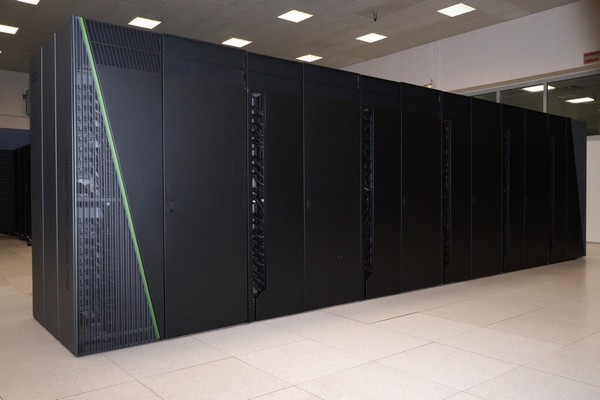
\includegraphics[height=5cm]{turing}
  }
  \begin{onlyenv}<2>
    \begin{tabular}{|r|r|r|r|}
  \hline
  \# nodes & Data             & T (s)        & Aggregated BW \\
  \hline\hline
  2        & 13.5Go           & 2.7      & 6.8Go/s \\
  4        & 27Go             & 2.9      & 9.3Go/s \\
    \vdots & \vdots           & \vdots   & \vdots  \\                                         
  64       & 430Go            & 4.1      & 105Go/s \\
  128      & 861Go            & 8.9      &  96Go/s \\
  256      & 1.7To            & 13.0     & 130Go/s \\
  512      & 3.4To            & 13.7     & 248Go/s \\
  1024     & 6.9To            & 15.9     & 434Go/s \\
  2048     & 13.4To           & 17.0     & 788Go/s \\
  4096     & 27.5To           & 18.7     & 1470Go/s \\
    \hline
    \end{tabular}
  \end{onlyenv}
\end{overlayarea}

\end{frame}



%%%%%%%%%%%%%%%%%%%%%%%%%%%%%%%%%%%%%%%%%%%%%%%%%%%%


\begin{frame}[fragile]
\frametitle{MPI : Reduce}

\begin{minted}[fontsize=\scriptsize]{C}
int MPI_Reduce(const void *sendbuf, void *recvbuf, int count,
               MPI_Datatype datatype, MPI_Op op, int root,
               MPI_Comm comm);
\end{minted}
               
\bigskip

\begin{center}
\begin{tikzpicture}[scale=0.5, >=latex]
%Bcast
\begin{scope}
  \begin{scope}
    \foreach \i in {0,1,...,6} {
      \draw[thick] (\i, 0) -- +(0, 6);
      \draw[thick] (0, \i) -- +(6, 0);
    }
    \node at (0.5, 5.5) {$\scriptscriptstyle \sum a_i$};
    \node at (1.5, 5.5) {$\scriptscriptstyle \sum b_i$};
    \node at (2.5, 5.5) {$\scriptscriptstyle \sum c_i$};
    \node at (3.5, 5.5) {$\scriptscriptstyle \sum d_i$};
    \node at (4.5, 5.5) {$\scriptscriptstyle \sum e_i$};
    \node at (5.5, 5.5) {$\scriptscriptstyle \sum f_i$};

  \end{scope}

\draw[ultra thick,<-] (7, 3) -- node[above] {Reduce} (11, 3);

\begin{scope}[xshift=12cm]
  \foreach \i in {0,1,...,6} {
    \draw[thick] (\i, 0) -- +(0, 6);
    \draw[thick] (0, \i) -- +(6, 0);
  }
  \foreach \i in {0,1,...,5} {
    \node at (0.5, 5.5-\i) {$a_\i$};
    \node at (1.5, 5.5-\i) {$b_\i$};
    \node at (2.5, 5.5-\i) {$c_\i$};
    \node at (3.5, 5.5-\i) {$d_\i$};
    \node at (4.5, 5.5-\i) {$e_\i$};
    \node at (5.5, 5.5-\i) {$f_\i$};
  }
\end{scope}
\end{scope}
\end{tikzpicture}
\end{center}

\begin{itemize}
\item Opérations prédéfinies : $+$, $\times$, $\min$, $\max$, et, ou, non, ...  
\item Opérations définissables par l'utilisateur
\end{itemize}
\end{frame}

%%%%%%%%%%%%%%%%%%%%%%%%%%%%%%%%%%%%%%%%%%%%%%%%%

\begin{frame}[fragile]
\frametitle{MPI : AllReduce}

\begin{minted}[fontsize=\scriptsize]{C}
int MPI_Allreduce(const void *sendbuf, void *recvbuf, int count,
                 MPI_Datatype datatype, MPI_Op op, MPI_Comm comm);
\end{minted}
               
\bigskip

\begin{center}
\begin{tikzpicture}[scale=0.5, >=latex]
%Bcast
\begin{scope}
  \begin{scope}
    \foreach \i in {0,1,...,6} {
      \draw[thick] (\i, 0) -- +(0, 6);
      \draw[thick] (0, \i) -- +(6, 0);
    }
  \foreach \i in {0,1,...,5} {
    \node at (0.5, 5.5-\i) {$\scriptscriptstyle \sum a_i$};
    \node at (1.5, 5.5-\i) {$\scriptscriptstyle \sum b_i$};
    \node at (2.5, 5.5-\i) {$\scriptscriptstyle \sum c_i$};
    \node at (3.5, 5.5-\i) {$\scriptscriptstyle \sum d_i$};
    \node at (4.5, 5.5-\i) {$\scriptscriptstyle \sum e_i$};
    \node at (5.5, 5.5-\i) {$\scriptscriptstyle \sum f_i$};
  }
  \end{scope}

\draw[ultra thick,<-] (7, 3) -- node[above] {AllReduce} (11, 3);

\begin{scope}[xshift=12cm]
  \foreach \i in {0,1,...,6} {
    \draw[thick] (\i, 0) -- +(0, 6);
    \draw[thick] (0, \i) -- +(6, 0);
  }
  \foreach \i in {0,1,...,5} {
    \node at (0.5, 5.5-\i) {$a_\i$};
    \node at (1.5, 5.5-\i) {$b_\i$};
    \node at (2.5, 5.5-\i) {$c_\i$};
    \node at (3.5, 5.5-\i) {$d_\i$};
    \node at (4.5, 5.5-\i) {$e_\i$};
    \node at (5.5, 5.5-\i) {$f_\i$};
  }
\end{scope}
\end{scope}
\end{tikzpicture}
\end{center}

\begin{itemize}
\item Opérations prédéfinies : $+$, $\times$, $\min$, $\max$, et, ou, non, ...  
\item Opérations définissables par l'utilisateur
\end{itemize}
\end{frame}

%%%%%%%%%%%%%%%%%%%%%%%%%%%%%%%%%%%%%%%%%%%%%%%%%%%%%%%%%%%%%%%%

\begin{frame}[fragile]
\frametitle{MPI : Reduce-Scatter}

\begin{minted}[fontsize=\scriptsize]{C}
int MPI_Reduce_scatter_block(const void* sendbuf, void* recvbuf,
                             int recvcount, MPI_Datatype datatype,
                             MPI_Op op, MPI_Comm comm)
\end{minted}
               
\bigskip

\begin{center}
\begin{tikzpicture}[scale=0.5, >=latex]
%Bcast
\begin{scope}
  \begin{scope}
    \foreach \i in {0,1,...,6} {
      \draw[thick] (\i, 0) -- +(0, 6);
      \draw[thick] (0, \i) -- +(6, 0);
    }
    
    \node at (0.5, 5.5) {$\scriptscriptstyle \sum a_i$};
    \node at (0.5, 4.5) {$\scriptscriptstyle \sum b_i$};
    \node at (0.5, 3.5) {$\scriptscriptstyle \sum c_i$};
    \node at (0.5, 2.5) {$\scriptscriptstyle \sum d_i$};
    \node at (0.5, 1.5) {$\scriptscriptstyle \sum e_i$};
    \node at (0.5, 0.5) {$\scriptscriptstyle \sum f_i$};
  \end{scope}

\draw[ultra thick,<-] (7, 3) -- node[above] {Reduce-Scatter} (11, 3);

\begin{scope}[xshift=12cm]
  \foreach \i in {0,1,...,6} {
    \draw[thick] (\i, 0) -- +(0, 6);
    \draw[thick] (0, \i) -- +(6, 0);
  }
  \foreach \i in {0,1,...,5} {
    \node at (0.5, 5.5-\i) {$a_\i$};
    \node at (1.5, 5.5-\i) {$b_\i$};
    \node at (2.5, 5.5-\i) {$c_\i$};
    \node at (3.5, 5.5-\i) {$d_\i$};
    \node at (4.5, 5.5-\i) {$e_\i$};
    \node at (5.5, 5.5-\i) {$f_\i$};
  }
\end{scope}
\end{scope}
\end{tikzpicture}
\end{center}

\begin{itemize}
\item Opérations prédéfinies : $+$, $\times$, $\min$, $\max$, et, ou, non, ...  
\item Opérations définissables par l'utilisateur
\item See also : \mintinline{C}{MPI_Reduce_scatter}
\end{itemize}
\end{frame}

%%%%%%%%%%%%%%%%%%%%%%%%%%%%%%%%%%%%%%%%%%%%%%%%%%%%%%%%%%%%%%%%%%%%%%%%%

\begin{frame}[fragile]
\frametitle{MPI : Scan}
\framesubtitle{A.k.a. Prefix-sum}

\begin{minted}[fontsize=\scriptsize]{C}
int MPI_Scan(const void* sendbuf, void* recvbuf, int count,
             MPI_Datatype datatype, MPI_Op op, MPI_Comm comm);
\end{minted}
               
\bigskip

\begin{center}
\begin{tikzpicture}[scale=0.5, >=latex]
%Bcast
\begin{scope}
  \begin{scope}
    \draw[thick] (0, 0) rectangle +(9, 6);
    \draw[thick] (3, 0) -- +(0, 6);
    \draw[thick] (6, 0) -- +(0, 6);
    \foreach \i in {0,1,...,6} {
      \draw[thick] (0, \i) -- +(9, 0);
    }
    
    \node at (1.5, 5.5) {$\scriptstyle a_0$};
    \node at (4.5, 5.5) {$\scriptstyle b_0$};
    \node at (7.5, 5.5) {$\scriptstyle c_0$};

    \node at (1.5, 4.5) {$\scriptstyle a_0 + a_1$};
    \node at (4.5, 4.5) {$\scriptstyle b_0 + b_1$};
    \node at (7.5, 4.5) {$\scriptstyle c_0 + c_1$};

    
    \node at (1.5, 3.5) {$\scriptstyle a_0 + a_1 + a_2$};
    \node at (4.5, 3.5) {$\scriptstyle b_0 + b_1 + b_2$};
    \node at (7.5, 3.5) {$\scriptstyle c_0 + c_1 + c_2$};

    \foreach \i in {3, 4, 5} {
      \node at (1.5, 5.5-\i) {$\scriptstyle a_0 + \dots + a_\i$};
      \node at (4.5, 5.5-\i) {$\scriptstyle b_0 + \dots + b_\i$};
      \node at (7.5, 5.5-\i) {$\scriptstyle c_0 + \dots + c_\i$};
    }
  \end{scope}

\draw[ultra thick,<-] (9.5, 3) -- node[above] {Scan} (11.5, 3);

\begin{scope}[xshift=12cm]
    \draw[thick] (0, 0) rectangle +(9, 6);
    \draw[thick] (3, 0) -- +(0, 6);
    \draw[thick] (6, 0) -- +(0, 6);
    \foreach \i in {0,1,...,6} {
      \draw[thick] (0, \i) -- +(9, 0);
    }

  \foreach \i in {0,1,...,5} {
    \node at (1.5, 5.5-\i) {$\scriptstyle a_\i$};
    \node at (4.5, 5.5-\i) {$\scriptstyle b_\i$};
    \node at (7.5, 5.5-\i) {$\scriptstyle c_\i$};
  }
\end{scope}
\end{scope}
\end{tikzpicture}
\end{center}

\begin{itemize}
\item Opérations prédéfinies : $+$, $\times$, $\min$, $\max$, et, ou, non, ...  
\item Opérations définissables par l'utilisateur
\item See also : \mintinline{C}{MPI_Exscan}
\end{itemize}
\end{frame}

%%%%%%%%%%%%%%%%%%%%%%%%%%%%%%%%%%%%%%%%%%%%%%%%%%%%%%%%%%%%%%%%%%%%%%%%%%%%%%

\begin{frame}[fragile]
\frametitle{MPI\_IN\_PLACE}

\begin{itemize}
\item Certaines opérations collectives doivent copier des données du buffer
  de départ vers le buffer de destination.

\item Au moins sur \texttt{root}, parfois chez tout le monde.
\end{itemize}

\begin{alertblock}{Pénible ?}
\begin{itemize}
\item \verb|MPI_IN_PLACE| à la place du buffer d'envoi désactive la copie.

\item Les données sont \emph{lues} (et écrites) dans le buffer de destination, là
  où elles auraient dû arriver. 

\item Fonctionne dans Scatter, Gather, Allgather, All-to-all, reduce, scan, etc.
\end{itemize}
\end{alertblock}
\end{frame}

%%%%%%%%%%%%%%%%%%%%%%%%%%%%%%%%%%%%%%%%%%%%%%%%%%%%%%%%%%%%%%%%%%%%%%%%%%%%%% 

\begin{frame}[fragile]
\frametitle{Un aspect pratique}

\begin{itemize}
\item \verb|MPI_Scatter| / \verb|MPI_Gather| / \verb|MPI_Alltoall| / \dots
  \begin{itemize}
  \item Même taille envoyée/reçue par tout le monde
  \item Très pratique si $N ~ \% ~ p = 0$.
  \end{itemize}
\end{itemize}

\medskip

\begin{alertblock}{Si $N ~ \% ~ p \neq 0$ ?}
\begin{itemize}
\item \verb|MPI_Scatterv| / \verb|MPI_Gatherv| /  \verb|MPI_Alltoallv| / \dots
  \begin{itemize}
  \item Tailles individualisées (mais encore plus d'arguments !)
  \end{itemize}
  
\medskip
  
\item Solution de facilité : bourrage
  \begin{itemize}
  \item Augmenter $N$ jusqu'à $p \lceil N/p \rceil$ en rajoutant... des zéros ? 
  \item Chaque \og tranche \fg de taille $\lceil N/p \rceil$.
  \item La dernière contient une portion inutile.
  \end{itemize}

\end{itemize}
\end{alertblock}
\end{frame}

%%%%%%%%%%%%%%%%%%%%%%%%%%%%%%%%%%%%%%%%%%%%%%%%%%%%%%%%%%%%%%%%%%%%%%%%%%

\begin{frame}
\frametitle{Sujets non abordés}

\begin{itemize}
\item Types personnalisés
\item IO parallèle
\item One-sided communications
  \begin{itemize}
  \item Mais on verra peut-être OpenSHMEM
  \end{itemize}
\item Création/gestion des intra/inter-communicateurs
\item Opérations collectives asynchrones
\item $\dots$
\end{itemize}

\bigskip
\pause
\Huge RTFM
\end{frame}

\end{document}

%%% Local Variables:
%%% TeX-command-extra-options: "-shell-escape"
%%% TeX-engine: xetex
%%% End: